%%%%%%FRONTESPIZIO%%%%%%
\begin{titlepage} % Suppresses headers and footers on the title page

    \setstretch{1.15}
    \centering % Centre everything on the title page

    % \scshape % Use small caps for all text on the title page

    \vspace*{\baselineskip}
    \begin{figure}[!h]
        \centering
        
\includegraphics[width=0.3\textwidth]{../titlepage/images/UNIPD.png}
    \end{figure}
    \vspace*{\baselineskip}

    \noindent\parbox{\textwidth}{\fontsize{15}{18}\selectfont\centering
    Università degli Studi di Padova\\
    Dipartimento di Fisica e Astronomia\\
    Advanced Physics Laboratory}%{\fontsize{13}{15}\selectfont bar!}
    % {\Large Università degli Studi di Padova}

    %\vspace*{2mm}
    %{\Large Dipartimento di Fisica e Astronomia}

	% \rule{\textwidth}{1.6pt}\vspace*{-\baselineskip}\vspace*{2pt} % Thick horizontal rule
	% \rule{\textwidth}{0.4pt} % Thin horizontal rule


    \vspace*{1cm}
    %{\Large Advanced Physics Laboratory}

    %\vspace*{2mm}
	%\textbf{\LARGE Rutherford Scattering} % Title

    {\fontsize{25}{30}\selectfont\bfseries Rutherford Scattering}

    \vspace{0.75\baselineskip} % Whitespace below the title


    \vspace*{\baselineskip}
    % \begin{figure}[!h]
    %     \centering
    %     
\includegraphics[width=0.4\textwidth]{../titlepage/images/NUCLEAR.jpg}
    % \end{figure}
    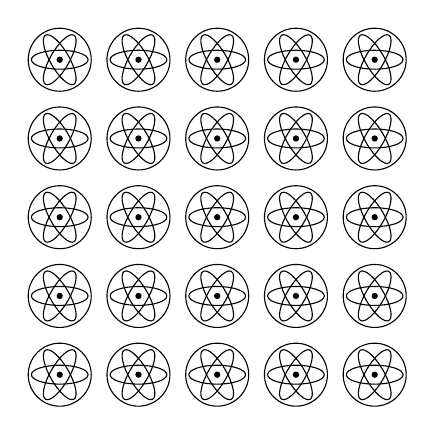
\begin{tikzpicture}[
        >=latex,
        font=\sffamily,
        atom/.style = {
            circle, minimum size=#1,
            append after command=
            {%
                \pgfextra{
                    \foreach \ang in {0,120,240}
                    \draw[rotate around={\ang:(0,0)}] (\tikzlastnode.center) ellipse (0.45*#1 and 0.15*#1);
                    \fill (\tikzlastnode.center) circle (0.05*#1);
                }
            }
        }
    ]
        \node[draw, atom=8mm] (C11) at (-2, 2){};
        \node[draw, atom=8mm] (C12) at (-1, 2){};
        \node[draw, atom=8mm] (C13) at ( 0, 2){};
        \node[draw, atom=8mm] (C14) at ( 1, 2){};
        \node[draw, atom=8mm] (C15) at ( 2, 2){};

        \node[draw, atom=8mm] (C21) at (-2, 1){};
        \node[draw, atom=8mm] (C22) at (-1, 1){};
        \node[draw, atom=8mm] (C23) at ( 0, 1){};
        \node[draw, atom=8mm] (C24) at ( 1, 1){};
        \node[draw, atom=8mm] (C25) at ( 2, 1){};

        \node[draw, atom=8mm] (C31) at (-2, 0){};
        \node[draw, atom=8mm] (C32) at (-1, 0){};
        \node[draw, atom=8mm] (C33) at ( 0, 0){};
        \node[draw, atom=8mm] (C34) at ( 1, 0){};
        \node[draw, atom=8mm] (C35) at ( 2, 0){};

        \node[draw, atom=8mm] (C41) at (-2,-1){};
        \node[draw, atom=8mm] (C42) at (-1,-1){};
        \node[draw, atom=8mm] (C43) at ( 0,-1){};
        \node[draw, atom=8mm] (C44) at ( 1,-1){};
        \node[draw, atom=8mm] (C45) at ( 2,-1){};

        \node[draw, atom=8mm] (C51) at (-2,-2){};
        \node[draw, atom=8mm] (C52) at (-1,-2){};
        \node[draw, atom=8mm] (C53) at ( 0,-2){};
        \node[draw, atom=8mm] (C54) at ( 1,-2){};
        \node[draw, atom=8mm] (C55) at ( 2,-2){};
    \end{tikzpicture}
    \vspace*{\baselineskip}

    \vspace*{\fill} % Whitespace between editor names and publisher logo

    \begin{minipage}[t]{0.4\textwidth}
        \begin{flushleft} \large
            \textsc{\textbf{Authors:}}\\
            %\href{http://www.johnsmith.com}{AAAA} % Author name - remove the \href bracket to remove the link
            {Ardino Rocco}\\
            {Mat. 1231629}\\
            \vspace{1mm}
            {Bortolato Gabriele}\\
            {Mat. ???????}\\
            \vspace{1mm}
            {Valente Alessandro}\\
            {Mat. ???????}
        \end{flushleft}
    \end{minipage}
    \hfill
    \begin{minipage}[t]{0.4\textwidth}
        \begin{flushright} \large
            \textsc{\textbf{Supervisor:}} \\
            %\href{http://www.jamessmith.com}{AAAA} % Supervisor name - remove the \href bracket to remove the link
            {Prof. Gianmaria Collazuol}
        \end{flushright}
    \end{minipage}\\[1cm]

\end{titlepage}

\clearpage{\pagestyle{empty}\cleardoublepage}
